\documentclass[11pt,letterpaper]{article}
\usepackage{naaclhlt2012}
\usepackage{times}
\usepackage{latexsym}
\usepackage{amsmath}
\usepackage{multirow}
\setlength\titlebox{1.65 cm}    % Expanding the titlebox
\usepackage{url}
\usepackage{color}
\usepackage{colortbl}
\usepackage[vlined,figure]{algorithm2e}
\usepackage{graphicx} 

\DeclareMathOperator*{\argmax}{arg\,max}

\definecolor{red}{rgb}{1,0,0}
\definecolor{lightgray}{cmyk}{0,0,0,.08}

\newcommand{\mnote}[1]{\marginpar{%
  \vskip-\baselineskip
  \raggedright\footnotesize
  \itshape\hrule\smallskip\tiny{#1}\par\smallskip\hrule}}  

%\newcommand{\mtodo}[1]{}
\newcommand{\mtodo}[1]{\mnote{\textcolor{red}{#1}}}
\newcommand{\red}[1]{\textcolor{red}{#1}}
\newcommand{\todo}[1]{\textcolor{red}{TODO: #1}}
\newcommand{\todop}[2]{\noindent\textcolor{red}{TODO for #1:} #2\\}
\newcommand{\todopi}[2]{[\textcolor{red}{TODO for #1:} #2]}
\newcommand{\secref}[1]{Section~\ref{#1}}
\newcommand{\tabref}[1]{Table~\ref{#1}}
\newcommand{\figref}[1]{Figure~\ref{#1}}
\newcommand{\code}[1]{{\small \tt #1}}
\newcommand{\emq}[1]{\emph{``#1''}}
\newcommand{\paraheader}[1]{\vskip 0.05in \noindent\emph{#1}}
\newcommand{\skipheader}{\vskip 0.05in}

\newcommand{\bm}{\boldsymbol}
\def\bs#1{\boldsymbol{#1}}

\newenvironment{my_itemize}{
\begin{itemize}
  \setlength{\itemsep}{2pt}
  \setlength{\parskip}{2pt}
  \setlength{\parsep}{1pt}}{\end{itemize}
}


\title{Learning a Reordering Model Without Parallel Data}

%\author{}
% \author{Alex Klementiev \ \ \ \  Ann Irvine \ \ \ \ Chris Callison-Burch \ \ \ \ David Yarowsky \\
% Center for Language and Speech Processing \\ Johns Hopkins University}

%\author{Author 1\\
%	    XYZ Company\\
%	    111 Anywhere Street\\
%	    Mytown, NY 10000, USA\\
%	    {\tt author1@xyz.org}
%	  \And
%	Author 2\\
%  	ABC University\\
%  	900 Main Street\\
%  	Ourcity, PQ, Canada A1A 1T2\\
%  {\tt author2@abc.ca}}

\date{}

\begin{document}
\maketitle

\begin{abstract}
The parameters of statistical models of translation are typically estimated from large bilingual parallel corpora.  However, these resources are expensive to create and are not available for most language pairs.  In this work we consider estimating reordering probabilities for a given set of phrase pairs using independent, monolingual corpora for the source and target languages. We propose a novel algorithm and show that using a monolingually estimated reordering model approaches the performance of the bilingually estimated model for Spanish to English and Urdu to English translation.
\end{abstract}

% ------------------------------------------------
\section{Introduction}

Given some input source language text, machine translation (MT) systems do the following: (1) choose corresponding target language words (or phrases or tree fragments), and (2) put them in the correct, grammatical order for the target language. Nearly all state of the art MT systems use sentence aligned parallel text to train models for doing both. However, such data does not exist for the majority of the world's languages and it is expensive to create. Developing a statistical MT system which does not depend on parallel text would allow us to build systems for translating languages which are out of reach for current models and existing data. 

In Anonymous (2012), we presented our results estimating phrase pair translation probabilities (the first MT task) from source and target monolingual corpora, which are relatively plentiful and easy to collect. In this work, we use the same monolingual corpora to estimate reordering probabilities. We assume that a phrase table is given and only estimate the reordering model. This allows us to directly compare our monolingually estimated reordering model with a standard bilingually estimated reordering model.

%MT: (1) choose words (phrases) in the target language, (2) put them in the right order.  Both need parallel data, which is expensive.  In this work, we address the reordering problem using monolingual data alone, which is cheap and plentiful.  In this work, we assume that a phrase table is \emph{given} and only estimate the reordering features.  We study how the induced reordering model compares with its standard counterpart induced from parallel data.

% ------------------------------------------------
\section{Background} \label{sect:bckg}

%\mtodo{Brief background on MT, reordering models.}

Statistical machine translation (SMT) was first formulated as a series of probabilistic models that learn word-to-word correspondences from sentence-aligned bilingual parallel corpora \cite{Brown:1993}.  \nocite{Brown1988}
%
Current methods, including {\em phrase-based} \cite{Och:2002,Koehn:2003} and {\em hierarchical} models \cite{Chiang:2005}, typically start by word-aligning a bilingual parallel corpus \cite{Och2003}.  They extract multi-word phrases that are consistent with the Viterbi word alignments, and use these phrases to build new translations.  Model parameters are estimated from large amounts of bitext.  One of those parameters is the reordering model

In phrase-baesd machine translation, each phrase pair $(e, f)$ has reordering parameters $p_o(\textnormal{orientation}|f,e)$ which indicate the distribution of its orientation with respect to the previously translated phrase. Orientations are {\it monotone, swap, discontinuous} \cite{tillman:2004:HLTNAACL,Kumar2004,Koehn-EtAl:2005:IWSLT}, see \figref{fig:reorderfeats}. 

In this work, we keep the definition of phrase-based reordering features, but estimate them from source and target language monolingual corpora alone. %In Section \ref{sect:order}, we introduce our novel algorithm, and in Section \ref{sect:eval} we evaluate its performance in end-to-end MT. 



% ------------------------------------------------
\section{Monolingual Reordering Estimation} \label{sect:order}

Here we introduce a novel algorithm for estimating $p_o(\textnormal{orientation}|f,e)$ from two monolingual corpora instead a bitext.

Figure \ref{fig:reorderfeats} illustrates how the phrase pair orientation statistics are estimated in the standard phrase-based SMT pipeline.  For a phrase pair like ($f =$ \emq{Profils}, $e =$ \emq{profile}), we count its orientation with the previously translated phrase pair ($f' =$ \emq{in Facebook}, $e' =$ \emq{Facebook}) across all translated sentence pairs in the bitext.  




\begin{figure}[t*]
\begin{center}
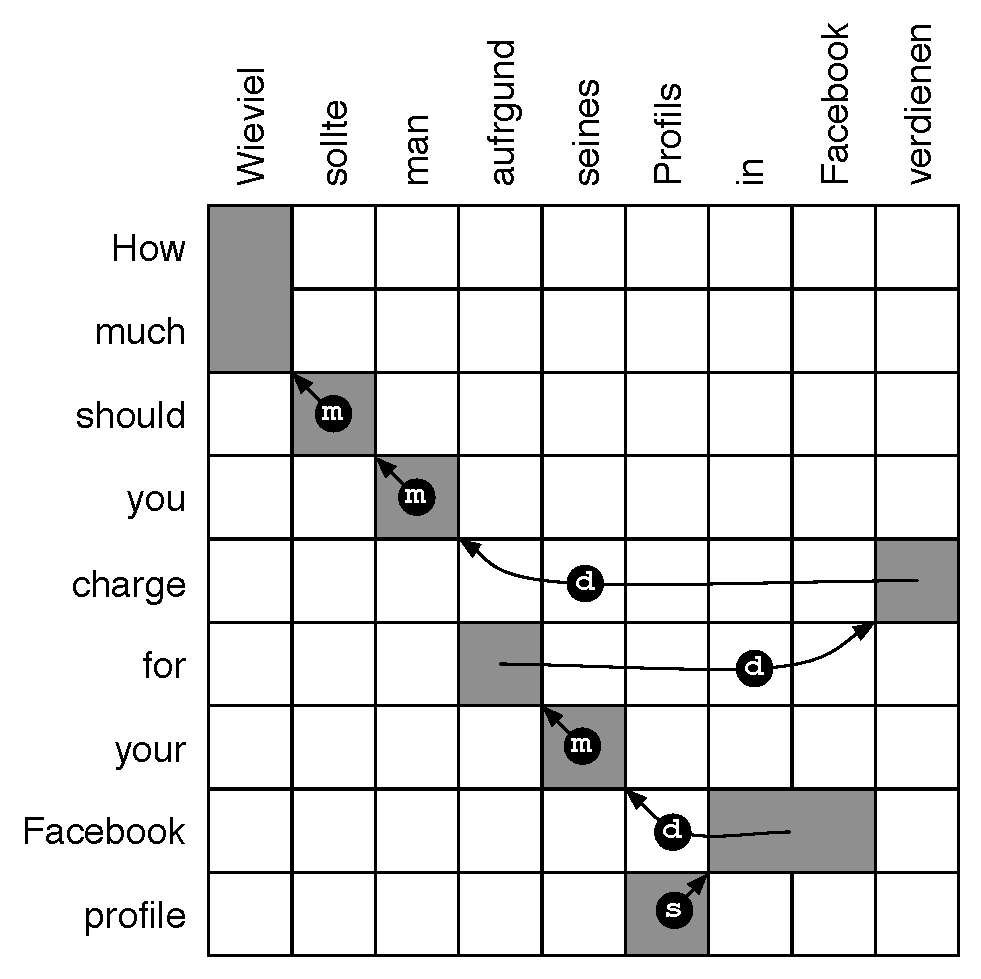
\includegraphics[width=0.8 \linewidth]{../figures/reorderfeats/reorderfeats.pdf}
\caption{The reordering probabilities from the phrase-based models are estimated from bilingual data by calculating how often in the parallel corpus a phrase pair $(f, e)$ is orientated with the preceding phrase pair in the 3 types of orientations (monotone, swapped, and discontinuous). }
\label{fig:reorderfeats} 
\end{center}
\vskip -0.2in
\end{figure}

\begin{figure}[t*]
%\vskip 0.1in
\begin{center}
%\vspace{-.85cm}
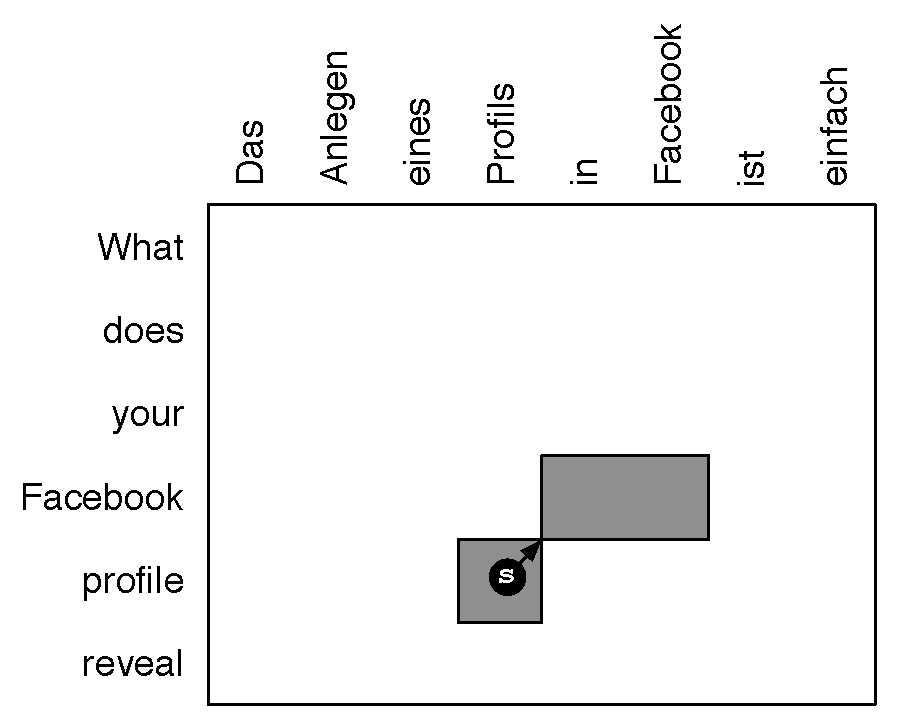
\includegraphics[width=0.8 \linewidth]{../figures/monoreord/monoreord.pdf}
%\vspace{-.25cm}
\caption{Collecting phrase orientation statistics for a English-German phrase pair (\emq{profile}, \emq{Profils}) from non-parallel sentences (the German sentence translates as  \emq{Creating a Facebook profile is easy}). %The longest preceding phrase \emq{Facebook} in source, has a phrase table translation \emq{in Facebook} appearing after the target phrase.
}
\label{fig:monoreord}
\end{center}
\vskip -0.2in
\end{figure}

In our setup we do not have translated sentence pairs.  Instead, we look for monolingual sentences in the source corpus which contain the source language phrase that we are interested in, like $f =$ \emq{Profils}, and at least one other nearby (contextual) source phrase that we have a translation for, like $f' =$ \emq{in Facebook}.  We then look for all target language sentences in the target monolingual corpus that contain the translation of $f$ (here $e =$ \emq{profile}) and any translation of $f'$.  \figref{fig:monoreord} illustrates that it is possible to find evidence for $p_o(\textnormal{swapped}| \it{ Profils},\it{ profile})$, even from the non-parallel, non-translated sentences drawn from two independent monolingual corpora.  By looking for foreign sentences containing pairs of adjacent foreign phrases $(f, f')$ and English sentences containing their corresponding translations $(e, e')$, we are able to increment orientation counts for $(f, e)$ by looking at whether $e$ and $e'$ are adjacent, swapped, or discontinuous, much in the same way as in Fig.~\ref{fig:reorderfeats}.







\SetAlFnt{\relsize{-1.5}}

\begin{algorithm}[t]

 \SetKwFunction{CollectOccurs}{CollectOccurs}
 \SetKwFunction{CollectPreceding}{CollectPreceding}
 \SetKwFunction{CollectFollowing}{CollectFollowing}
 \SetKwFunction{CollectDisc}{CollectDisc}
 \SetKwBlock{Body}{}{}
 \SetCommentSty{text}
 \SetFuncSty{text}

 \hrule \vskip 0.2cm

  \KwIn{Source and target phrases $f$ and $e$,\\
  \hskip 0.85cm Source and target monolingual corpora $\emph{C}_f$ and $\emph{C}_e$,\\
  \hskip 0.85cm Phrase table pairs $\emph{T} = \{(f^{(i)}, e^{(i)})\}_{i=1}^{N}$.
  } 
  \KwOut{Orientation features ($p_m, p_s, p_d$).}
  
  \vskip 0.2cm \hrule \vskip 0.2cm

  $S_f \leftarrow$ sentences containing $f$ in $\emph{C}_f$\;
  $S_e \leftarrow$ sentences containing $e$ in $\emph{C}_e$\;
  
  $(B_f, -, -) \leftarrow \CollectOccurs(f, \cup_{i=1}^{N} f^{(i)}, S_f)$\;
  $(B_e, A_e, D_e) \leftarrow \CollectOccurs(e, \cup_{i=1}^{N} e^{(i)}, S_e)$\;
    
  $c_m = c_s = c_d = 0$\;
  
  \vskip 0.1cm 

  \ForEach{unique $f'$ in $B_f$} {
    \ForEach{translation $e'$ of $f'$ in $\emph{T}$} {

      $c_m = c_m + \#_{B_e}(e')$\; 
       $c_s = c_s + \#_{A_e}(e')$\; 
       $c_d = c_d + \#_{D_e}(e')$\; 
    }
  }
  
  $c \leftarrow c_m + c_s + c_d$;
    
  \Return{$({c_m \over c}, {c_s \over c}, {c_d \over c})$}

  \vskip 0.2cm \hrule \vskip 0.2cm

  \CollectOccurs{$r$, $R$, $S$} \Body{
   $B \leftarrow ()$; $A \leftarrow ()$; $D \leftarrow ()$\;

    \ForEach{sentence $s \in S$} {
      \ForEach{occurrence of phrase $r$ in $s$} {
        $B \leftarrow B$ $\cup$ \CollectPreceding{$r$, $R$}\;
        $A \leftarrow A$ $\cup$ \CollectFollowing{$r$, $R$}\;
        $D \leftarrow D$ $\cup$ \CollectDisc{$r$, $R$}\;
      }
    }
    
    \Return{($B$, $A$, $D$)}\;
  }
  
  \vskip 0.2cm \hrule \vskip 0.2cm

  \caption{Algorithm for estimating reordering probabilities from monolingual data.} \label{fig:algoreorder}
  \vskip -0.2in
\end{algorithm}


%In the phrase-based SMT pipeline, phrase pair orientation statistics are collected using word alignments.  We keep a similar reordering model formulation but infer its parameters from monolingual data instead.  The orientation information for a phrase pair ($f$, $e$) is collected from source and target sentences containing ($f$, $e$) as well as other phrase pairs.  Suppose one such sentence pair contains another pair of phrases ($f'$, $e'$), and that $f'$ is immediately adjacent to $f$.  The idea is to check whether $e'$ stays in the same order with $e$, swaps, or becomes discontinuous in the target sentence. Consider the simple example in \figref{fig:monoreord}: the phrase pair is ($f =$ \emq{profile}, $e =$ \emq{Profils}), and a given pair of non-parallel sentences also contains a phrase table entry ($f' =$ \emq{Facebook}, $e' =$ \emq{in Facebook}).  In this example, the phrase $f'$ preceding $f$ in the source sentence swaps order with $e$ in the target.  When we collect these counts over large monolingual corpora, we expect the swap, monotone, and discontinuous counts to provide good estimates for the orientation features (\figref{fig:algoreorder}).
%Note that multiple phrases may immediately precede $f$ and appear in the phrase table; however, we only use the longest of them to collect reordering counts.  

Figure \ref{fig:algoreorder} details our algorithm. Contextual phrases for some given source or target phrase \code{r} are only collected (in \code{CollectPreceding}, \code{CollectFollowing}, and \code{CollectDisc} on \figref{fig:algoreorder}) if they also have translations in our given phrase table \code{R}.  Note that shorter and more frequent phrases (e.g. punctuation) are more likely to appear in multiple orientations with a given phrase, and therefore provide poor evidence of re-ordering.  Therefore, when collecting contextual phrases for reordering feature estimation, we:

\begin{itemize}
  \item Keep only the longest contextual phrases (which also appear in the phrase table).
  \item Prune the set of phrases so that we only keep a small set of least frequent contextual phrases (this has the effect of dropping many function words and punctuation marks and and relying more heavily on multi-word content phrases to estimate the reordering).\footnote{The pruning step has an additional benefit of minimizing the memory needed for orientation feature estimations.}
  \item Do not look too far away from a given phrase when collecting discontinuous phrases in \code{CollectDisc}.
\end{itemize}

We empirically investigate the effect of all of these choices in \secref{sect:eval}.

% ------------------------------------------------
\section{Empirical Evaluation} \label{sect:eval}

In this work, we assume that a phrase table and corresponding phrase pair translation scores are given\footnote{In our experiments, the phrase table and translation probabilities are estimated using Europarl (Spanish) and NIST (Urdu) parallel corpora. However, in principle, they could be estimated using any method, including one that only makes use of monolingual corpora.}, but we estimate phrase pair reordering features from monolingual data.  We use our monolingually induced reordering model in place of its bilingually estimated counterpart in a complete phrase-based SMT pipeline, and we evaluate end-to-end performance using BLEU. 

The extent to which reordering models contribute to overall MT performance varies by language. For example, our standard phrase-based SMT model trained on the Spanish-English parallel Europarl corpus achieves a BLEU score of 21.87. Dropping the bilingually estimated orientation-based reordering model and using a distortion-based model, which does not require any parallel data for training, instead results in a BLEU score of 21.54, only about 0.3 BLEU less. Because the difference is so small, it is difficult to evaluate an alternative reordering model. For this reason, we report BLEU scores using our reordering model in combination with bilingually estimated phrase pair translation scores as well as using no phrase pair translation scores at all (``W/ Ph Feats'' and ``W/O Ph Feats'', respectively, in Table \ref{bleu-table}). The latter is closer to our ultimate goal of doing SMT without parallel text, in which case we will estimate reordering features as well as phrase pair translation scores using monolingual corpora.

%. \todo{i.e. experiments -/B, -/-. -/M and, possibly, B/B, B/-. B/M}.

\begin{table}[t]
\begin{smaller}
\begin{center}
\begin{tabular}{|c|c|c|c|c|c|}
\hline
Exp & Wdw & Long & Prop.  & W/ Ph & W/O Ph \\
Num & Size & Only? &  Dsc. & Feats  & Feats \\
\hline
\multicolumn{6}{|l|}{Spanish} \\
\hline
\multicolumn{4}{|l|}{Standard Biling. Reorder} & 21.87 & 21.54 \\ 
\hline
\multicolumn{4}{|l|}{Distortion Baseline} & 21.54 & 4.00 \\ 
\hline
1 & 3 & Y & 3x & {\bf 21.67} & {\bf 10.80} \\
\hline
2 & 3 & N & 3x & 21.68 & 9.46 \\
3 & 3 & Y & 1/10 & 21.44 & 9.85 \\
%4 & 3 & Y & Inf. &  &  \\
%5& 3 & N & 1/10 &  &  \\
%6& 3 & N & Inf. &  &  \\
%7& All & N & 3x &  &  \\
\hline
\multicolumn{4}{|l|}{Gain over baseline} & 0.13 & 6.80 \\ 
\hline
\hline
\multicolumn{6}{|l|}{Urdu} \\
\hline
\multicolumn{4}{|l|}{Standard Biling. Reorder} & 19.57 & 11.49 \\ 
\hline
\multicolumn{4}{|l|}{Distortion Baseline} & 16.89 & 10.04 \\
\hline
4 & 3 & Y & 3x & {\bf 17.23} & {\bf 9.50} \\
\hline
5 & 3 & N & 3x & 17.14 & 9.60 \\
6 & 3 & Y & 1/10 & 15.26 & 2.94 \\
7 & 3 & Y & Inf. & 17.04 & 9.53 \\
8 & 3 & N & 1/10 & 16.93 & 2.95 \\
9 & 3 & N & Inf. & 17.53 & 9.37 \\
10 & All & N & 3x & 17.00 & 8.52 \\
\hline
\multicolumn{4}{|l|}{Gain over baseline} & 0.34 & - \\ 
\hline
\end{tabular}
\end{center}
\vskip -0.1in
\caption{\label{bleu-table}BLEU score results on Spanish to English and Urdu to English translation. ``W/ Ph Feats'' refers to experiments using phrase pair translation scores estimated over parallel text and ``W/O Ph Feats'' refers to experiments using no phrase pair translation scores. Baseline (distortion-based reordering) and standard bilingually estimated model results are given. ``Wdw Size'' refers to the max distance between discontinuous phrases (`Inf' means phrase pairs can be maximally far apart within a sentence). ``Long Only?'' refers to whether or not the model considers only the longest contextual phrase in the window. ``Prop. Dsc.'' refers to the number of low frequency discontinuous phrases that the model considers relative to the number of preceding and following phrases, usually 500 phrases each.}
\vskip -0.15in
\end{smaller}
\end{table}


\paraheader{Data.} We estimate our reordering features using subsets of the Spanish and English Gigaword corpora\footnote{LDC2009T21 and LDC2009T13} for our Spanish MT experiments and from monolingual English and Urdu crawled web data for the our Urdu MT experiments. In all cases, we sampled about 1 million lines of each corpora with respect to the phrase table. Doing so ensured that the sampled sentences would be relevant for our phrases of interest and also minimized the computational time it took to compute the reordering models.

%\paraheader{Evaluation metrics.} %We evaluate the induced reordering both in the complete system and using the following metric. \todo{Define}.  Intuitively, it measures how well the monolingual reordering features agree with their bilingually estimated counterparts in their ordering preferences for a given phrase.

Table \ref{bleu-table} shows our experimental results. Our baseline is a simple distortion-based reordering model. Nearly all of our experimental conditions outperform the baseline, in some cases by a very wide margin. In the following discussions, we refer to the experiment numbers shown in the left column and vary several algorithmic parameters. The best configuration, experiments 1 (Spanish) and 4 (Urdu), are bold. %in Table \ref{bleu-table} are best. 

\subsection{Longest vs. All Phrases}
Here we compare results estimating reordering scores using (a) only the longest phrase (of those that we know how to translate) in the context of the given phrase of interest, $r$, and (b) all contextual phrases. We expect that using only the longest phrase will perform better because shorter, more frequent phrases are likely to appear in many positions relative to $r$. The Spanish results in Table \ref{bleu-table} show that when phrase translation scores aren't used, considering only the longest contextual phrase in estimating reordering scores (Exp 1) proved to be a better strategy than using all contextual phrases (Exp 2). However, the Urdu results (Exp 4-5) are about the same for each condition. This is likely due to the fact that the Urdu phrase table, which is estimated from a much smaller parallel text than the Spanish table, includes fewer long phrases.
%sparse so long phrases which we know how to translate (i.e. are in the phrase table) are not found in the context of a given Urdu phrase as often in Urdu monolingual text as in Spanish. 

\subsection{Pruning Contextual Phrases}
We perform experiments varying the {\it number} of contextual phrases that we collect for a given phrase of interest, $r$. In additional experiments (omitted due to space constraints), we found that collecting enough low frequency phrases to make good estimates but not so many that we include very frequent phrases, which are likely to occur in many positions in a sentence relative to $r$, works well. In particular, we found that considering $500$ preceding and following contextual phrases and $1500$, or three times as many discontinuous phrases, yields good results. Additionally, we find that the {\it proportion} between the number of collected discontinuous phrases and preceding/following phrases affects results more than absolute numbers. This makes sense; increasing the proportion of discontinuous phrases increases the model's general preference for discontinuous reorderings. Comparing Urdu experiment 4 with 6 and 7, and Spanish experiment 1 with 3, demonstrates performance drops, in some cases dramatically, both when (a) considering all discontinuous phrases, and (b) considering very few discontinuous phrases. %These results make sense; collecting a very small or huge amount of discontinuous phrases, relative to the other orientations, would result in relatively very high discontinuous reordering scores. 

\subsection{Collecting Discontinuous Phrases}
Finally, we vary the maximum allowed distance between our phrase of interest, $r$, and the discontinuous phrases that we collect. 
%In Table \ref{bleu-table}, we present one experiment for each language pair that demonstrates the decrease in performance that results when discontinuous phrases are collected from anywhere in a given sentence, rather than within a narrow window of words around the phrases of interest. 
When we collect discontinuous phrases from anywhere in the sentence instead of within a narrow window of words around $r$, performance drops (Urdu experiment 10).
%Urdu experiment 14, in contrast to 8, shows a modest drop in BLEU score under this condition when phrase translation scores are used and a larger drop when they are not. The same is shown in comparing Spanish experiment 7 with 1. 
Intuitively, this is what we expect. Discontinuous phrases located far away from our phrase of interest in a given sentence are unlikely to indicate anything about the reordering probabilities between the source and target phrases of interest.


\section{Conclusion}
In this work, we have presented a novel algorithm which is capable of estimating a phrase-based statistical machine translation reordering model from source and target independent, monolingual corpora. Spanish-English and Urdu-English reordering models estimated using the algorithm outperform a distortion-based baseline. This work is critical in moving away from SMT's current reliance on parallel corpora, and towards SMT systems that are estimated from monolingual data alone. %which are unavailable for many language pairs.

% ------------------------------------------------
%\section*{Acknowledgments}

%Do not number the acknowledgment section.

\vskip -0.1in

\bibliographystyle{naaclhlt2012}
\bibliography{reorder}

\end{document}
